\section{Methodology}
\label{sec:method}

\subsection{Framework Overview}

\begin{figure*}[t]
\centering
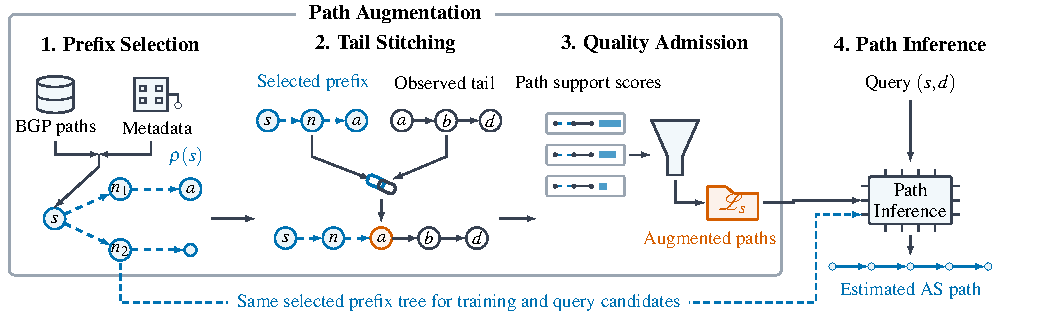
\includegraphics[width=\textwidth]{figures/fig2_overview.pdf}
\caption{\sys constructs a source-specific prefix tree, joins its prefixes
to observed tails, and selects an augmented path library. The same complete
tree constrains candidate generation during model training and inference;
the admitted library supplies both training labels and local path knowledge.}
\label{fig:overview}
\end{figure*}

\sys addresses source cold start by transferring routing evidence from
other networks. Its augmentation procedure, \pats (Prefix-Anchored Tail
Stitching), first selects likely forwarding neighbors and determines
whether to explore their next hops. It then joins the resulting prefixes
to intact observed tails and assesses the complete constructed routes.
The resulting library trains a source-specific inference model without
opening the source's held-out route labels. Figure~\ref{fig:overview}
shows the separation between path augmentation and final inference.

Two objects are retained for each source: the complete selected prefix
tree $\mathcal T_s$ and the admitted path library $\mathcal L_s$. They serve different
purposes. The tree defines the permitted early forwarding choices; the
library provides surrogate training routes and local path knowledge.
Candidate generation uses the complete tree, including selected prefixes
that do not happen to dominate the admitted library. Thus library
selection cannot silently redefine the source's permitted exits.

\subsection{Representing Heterogeneous Routing Evidence}
\label{sec:representation}

We represent public AS relationships and ASRank attributes,
PeeringDB presence, and independent BGP observations at AS-pair,
transition, and complete-path levels~\cite{CAIDA,caidaASrank,PeeringDB}.
Table~\ref{tab:method_features} summarizes their roles. Features are
tabular, with explicit missingness and conflict indicators. Shared
PeeringDB IXPs or facilities identify potential interconnection partners;
co-location alone does not establish a physical link or an export policy.

\begin{table}[t]
\centering
\caption{Evidence representations and their computational roles. Missing
and conflicting observations remain explicit.}
\label{tab:method_features}
\footnotesize
\begin{tabularx}{\columnwidth}{@{}lX@{}}
\toprule
Representation & Features and use\\
\midrule
AS pair & Public adjacency and commercial roles; ASRank degree, cone,
and network attributes; PeeringDB IXP/facility overlap and population;
independent edge support. Neighbor retrieval and ranking.\\
Graph structure & Common-neighbor overlap, Adamic--Adar,
resource allocation, role-conditioned bridges; source first- and
second-layer size. Structural ranking and $\rho(s)$.\\
Prefix/transition & Preceding, current, and next AS; local rank and
presence scores; edge provenance and possible commercial phases.
Conditional exploration and prefix-state tracking.\\
Path evidence (181) & Ordered path, suffix, edge and destination
support; AS count and commercial-role sequence; public endpoint context.
Base features for complete-path scoring.\\
Prefix reliability (32) & Support/missingness across added edges,
inferred-edge fraction, feasible phase states, and soft first-hop
transit-role evidence.\\
Actual next hop (9) & Conditional support, rank, missingness, and
phase status of the candidate's actual third AS.\\
Destination context (33) & Donor-source agreement and equally weighted
route fractions at the first hop and stitching boundary, with incoming-role
conditioning and explicit absent-boundary indicator.\\
\bottomrule
\end{tabularx}
\end{table}


\paragraph{Separating evidence from supervision.}
The upstream procedure masks complete observations by their original
first ASN before expanding paths into segments. Independent background
observations provide ordered edges and forward contiguous segments.
Task-source observations have separate roles: training origins provide
supervised labels and destination-conditioned donor statistics, while
held-out origins provide evaluation labels. A segment containing $s$
inside another origin's observation can remain evidence; an observation
originally rooted at held-out $s$ is excluded from this upstream evidence.
Tails preserve their observed direction and are never constructed by
reversing a route. These upstream guarantees apply to the explicitly
masked corpus; the provenance of inherited downstream graph and embedding
artifacts is assessed separately in the experimental protocol.

\paragraph{Destination-conditioned transfer.}
A path observed at an intermediate AS need not be exported to a particular
neighbor~\cite{rfc4271}. We therefore complement segment support with
evidence about which next hops other receivers observe toward the same
destination. For an original training donor $v$, let $c_v(n,a,d)$ count
distinct complete routes beginning $(v,n,a)$ and ending at $d$, and let
$c_v(n,d)=\sum_b c_v(n,b,d)$. With
$V_{n,d}=\{v:c_v(n,d)>0\}$, two representative features are
\begin{equation}
\begin{split}
f(n,a,d)&=\frac{|\{v\in V_{n,d}:c_v(n,a,d)>0\}|}{|V_{n,d}|},\\
m(n,a,d)&=\frac{1}{|V_{n,d}|}\sum_{v\in V_{n,d}}
                         \frac{c_v(n,a,d)}{c_v(n,d)}.
\end{split}
\label{eq:destination_evidence}
\end{equation}
The first measures agreement across donors and the second gives every
donor equal weight after normalizing its alternative routes. We also
condition these statistics on the donor's incoming commercial role at
$n$, matching the candidate receiver's role when it is known. This uses
original receiver contexts, rather than treating every internal occurrence
of $n$ as an independent receiver observation.

These features are evaluated at both the first-hop transition and the
construction boundary. Two 16-column context vectors and one boundary
indicator add 33 columns to 181 path-evidence, 32 prefix-reliability,
and nine actual-next-hop columns, giving a 255-column complete-path
representation. Missing donor coverage remains explicit. For a training
source, the entire original-source fold is removed from its donor
statistics, even when recursion changes the stitching anchor.

\subsection{Source-Conditioned Neighbor Selection and Exploration}
\label{sec:prefix_selection}

\paragraph{Learning likely forwarding choices.}
Candidate neighbors are retrieved from public or independently observed
adjacency and PeeringDB co-location, with graph-supported candidates
prioritized in a pool of at most 4,096 ASes. Two LightGBM
rankers~\cite{ke2017lightgbm} use a public-evidence view and a structurally
extended view. The latter adds common-neighbor overlap, Adamic--Adar,
resource-allocation, and population-weighted IXP/facility features.
Each view also has a binary presence head.

Training first-hop importance gives each destination equal weight,
divided among its distinct observed routes. Observed neighbors ranked
1--3, 4--10, and beyond ten receive relevance labels
3, 2, and 1; unobserved candidates receive 0. Presence indicates use in
this finite reference corpus. These targets measure observed routing
choices, rather than link existence or traffic volume.

Let $r_s^{\mathrm{pub}}(n),r_s^{\mathrm{str}}(n)$ denote the ranker outputs
and $p_s^{\mathrm{pub}}(n),p_s^{\mathrm{str}}(n)$ the presence outputs.
The protected core is
\begin{equation}
K_s=\operatorname{Top}_3(r_s^{\mathrm{pub}})
       \cup\operatorname{Top}_3(r_s^{\mathrm{str}}).
\label{eq:protected_core}
\end{equation}
For ordering within the core and the remaining candidates, we use
\begin{equation}
\begin{split}
\bar p_s(n)&=\tfrac12\bigl(p_s^{\mathrm{pub}}(n)+p_s^{\mathrm{str}}(n)\bigr),\\
u_s(n)&=z(r_s^{\mathrm{str}}(n))+
                   0.5\log\frac{\bar p_s(n)}{1-\bar p_s(n)},
\end{split}
\label{eq:neighbor_ranking}
\end{equation}
where $z$ standardizes within the candidate pool and presence outputs
are clipped to $[10^{-6},1-10^{-6}]$ before taking the logit.
The core precedes the remaining candidates, with descending $u_s$ and
ASN tie breaking. Presence outputs are uncalibrated observation-support
scores; we do not interpret them as forwarding probabilities.

\paragraph{Adapting exploration to source structure.}
Degree alone misses a source whose first hop conceals a large next-layer
choice set. Let $b_1(s)$ be the source's public degree, and let $b_2(s)$
count distinct second-layer ASes reachable through loop-free,
commercially non-incompatible two-hop public prefixes. Unknown roles
remain eligible. We define
\begin{equation}
\rho(s)=\frac{b_2(s)}{b_1(s)^2}.
\label{eq:source_rho}
\end{equation}
This is a structural control statistic, not a routing probability.
It is computed once for the original source and is not recomputed to
switch policies at its neighbors. A source with no usable public degree
remains unresolved.

When $\rho(s)\leq1$, we select the longest prefix of the protected-core
ordering containing $K_s$, limited to a root budget $\kappa$, whose mean
$\bar p_s$ is at least 0.7. If none qualifies, the core is retained with
uncertain support. For each selected neighbor $n$, we count usable
independent forward tails for $(s,n)$, stopping once 300 are found.
A usable direct prefix is retained. If its capacity is below 300,
exploration also proposes $(s,n,a)$ prefixes.
An explored child is retained only if it has at least one usable tail.
The evaluated protocol uses $\kappa=21$, the 90th-percentile number of
first-hop neighbors needed to cover 80\% of original training paths in
the February source statistics. This is a search budget, not a
guarantee of reference coverage for a new source.

When $\rho(s)>1$, only the dual-ranker core $K_s$ is selected, yielding
at most six roots. Every root is expanded to $(s,n,a)$ independently
of its direct-tail capacity. This exposes choices hidden behind a narrow
first layer; the high-$\rho$ branch does not retain a broad direct-tail
bypass. Both policies use the same next-hop width of ten and a maximum
prefix length of three ASes.

\paragraph{Prefix-aware next-hop prediction.}
A conditional ranker uses the preceding AS, current AS, and candidate
next AS to transfer local routing preferences. Its candidate pool is
limited to 512. Each proposed extension must avoid visited ASes and have
independent/public edge evidence, or co-location accompanied by a finite
learned support score. It must also preserve at least one feasible
commercial phase of the complete prefix. We track upward, post-peer,
and downward states; sibling edges are neutral and unknown relationships
retain all feasible states. Distinct prefixes and phase states sharing
an anchor remain distinct. This is local conditional transfer, not a
claim that multiplying local scores gives a calibrated path probability.
No supported continuation means stopping that branch rather than
inventing an extension.

\subsection{Prefix-Anchored Tail Construction}
\label{sec:construction}

For each selected prefix $q=(s,\ldots,z)$, \pats joins it to an intact
observed forward tail $t=(z,\ldots,d)$:
\begin{equation}
q\oplus t=(s,\ldots,z,\ldots,d),
\label{eq:pats_join}
\end{equation}
including the common anchor $z$ once. Reusing a tail preserves multiple
consecutive observed routing choices. It does not establish that $s$
would learn or select the resulting route.

Construction checks valid ASNs, 3--20 ASes, absence of loops, support
for each added prefix edge, and existence of a valley-free assignment
consistent with known relationships~\cite{gao2001inferring}. Missing
relationships are retained as unknown rather than automatically rejected.
The same physical path may arise from different prefixes; ordered
sequences are deduplicated while retaining their construction provenance.

To bound scoring work while preserving alternatives, construction keeps
up to two evidence-prioritized candidates per first hop, actual third AS,
destination, and AS count. It favors fewer unobserved prefix extensions
and stronger independent segment support. A deterministic hash ordering
selects 5,000 destination contexts, supplemented by all destinations of
direct prefixes covering at most 1,000 destinations and up to 50 protected
destinations per other explicit prefix. These are construction work
budgets, not a final library-size cap.

\subsection{Complete-Path Scoring and Library Admission}
\label{sec:admission}

\paragraph{Learning finite-observation support.}
A LightGBM classifier $h_\theta(\phi(P))$ assesses the 255-column
representation of a complete constructed path. For a training source,
an exact ordered match to its original reference is positive. A
nonmatching candidate is negative only if its destination has reference
coverage; candidates for uncovered destinations remain unlabeled.
The weighted binary objective balances training sources, first hops,
destinations within first hops, and alternatives within each context.
The model uses 300 trees, at most 31 leaves per tree, maximum depth seven,
and learning rate 0.04.

Models are fitted separately for each date using registered training
origins. Neighbor and transition predictions for a training source use
heads fitted without its original-source fold; destination features
exclude the same fold. This is stagewise source isolation. The final
path classifier is fitted on these training cases, and held-out source
routes never determine its features or parameters. Because non-observation
does not prove route impossibility, $h_\theta$ estimates support in a
finite observation corpus, rather than the probability of forwarding
reality.

\paragraph{Source-relative admission.}
Let $\mathcal B_s$ be the legal deduplicated source candidate pool and
$q(P)=h_\theta(\phi(P))$. We normalize within that source:
\begin{equation}
\widetilde q_s(P)=\frac{q(P)}{\max_{P'\in\mathcal B_s}q(P')}.
\label{eq:relative_quality}
\end{equation}
The nominal threshold is 0.75. To retain at least 1,000 paths when
positive-scored capacity permits, let $\widetilde q_{s,(1000)}$ be the
1,000th highest relative score and set
\begin{equation}
\begin{split}
\tau_s&=\min\{0.75,\widetilde q_{s,(1000)}\},\\
\mathcal L_s&=\{P\in\mathcal B_s:\widetilde q_s(P)\geq\tau_s\}.
\end{split}
\label{eq:quality_admission}
\end{equation}
All cutoff ties are retained and there is no upper size cap. The library
is unresolved if fewer than 1,000 legal paths exist, if the required
cutoff is zero, or if the source maximum is zero. The threshold relaxation
and actual cutoff are recorded. Relative quality is an admission ranking
criterion, not a guarantee of 75\% route accuracy. Algorithm~\ref{alg:path_synthesis}
summarizes augmentation.

\begin{algorithm}[t]
\caption{Prefix-Anchored Tail Stitching and Admission}
\label{alg:path_synthesis}
\footnotesize
\begin{algorithmic}[1]
\Require Source $s$, public topology $G$, independent tails $\mathcal T$
\Require Neighbor heads $g$, conditional ranker $g_c$, path scorer $h_\theta$
\Require Root budget $\kappa$ ($21$ in the evaluated protocol)
\Ensure Prefix tree $\mathcal T_s$ and admitted library $\mathcal L_s$, or unresolved
\If{$b_1(s)=0$}
  \State \Return unresolved
\EndIf
\State $\rho\gets b_2(s)/b_1(s)^2$
\State $K\gets\operatorname{Top}_3(g_{\rm pub}(s))\cup\operatorname{Top}_3(g_{\rm str}(s))$
\If{$\rho\leq1$}
  \State $N\gets\Call{ProtectedSupportPrefix}{s,K,\kappa,0.7}$
\Else
  \State $N\gets K$
\EndIf
\State $Q\gets\emptyset$
\ForAll{$n\in N$}
  \State $q\gets(s,n)$; $c\gets\Call{UsableTailCount}{q,\mathcal T,300}$
  \If{$\rho\leq1$ and $c>0$}
    \State $Q\gets Q\cup\{q\}$
  \EndIf
  \If{$\rho>1$ or $c<300$}
    \State $A\gets\Call{SupportedTopK}{g_c(s,q),10}$
    \ForAll{$a\in A$ with $a\notin q$}
      \State $q'\gets q\mathbin{\|}(a)$
      \If{$\rho>1$ or $\Call{UsableTailCount}{q',\mathcal T,1}>0$}
        \State $Q\gets Q\cup\{q'\}$
      \EndIf
    \EndFor
  \EndIf
\EndFor
\State $\mathcal T_s\gets\Call{PreservePrefixPhaseStates}{Q,G}$
\State $\mathcal B\gets\{q\oplus t:q\in Q,\ t\in\mathcal T_{\mathrm{last}(q)},\ \Call{ValidJoin}{q,t}\}$
\State $\mathcal B\gets\Call{ConstructionRepresentatives}{\mathcal B}$
\State $\mathcal B\gets\Call{ProtectedDestinationBudget}{\mathcal B}$
\State $(\mathcal B,q)\gets\Call{DeduplicateAndScore}{\mathcal B,h_\theta}$
\If{$|\mathcal B|<1000$ or $q_{(1000)}\leq0$}
  \State \Return unresolved \Comment{retain failure provenance}
\EndIf
\State $\widetilde q(P)\gets q(P)/\max_{P'\in\mathcal B}q(P')$
\State $\tau\gets\min\{0.75,\widetilde q_{(1000)}\}$
\State $\mathcal L_s\gets\{P\in\mathcal B:\widetilde q(P)\geq\tau\}$
\State \Return $\mathcal T_s,\mathcal L_s$ \Comment{retain all cutoff ties and path provenance}
\end{algorithmic}
\end{algorithm}


\subsection{Consistent Candidate Generation and Path Inference}
\label{sec:inference}

\paragraph{Reusing the complete tree.}
Training and query candidate generation both consume the same frozen
$\mathcal T_s$. For a destination $d$, each anchor supplies intact forward
observed tails toward $d$ and, when available, a shortest-path proposal
from the permitted topology. Every joined candidate is checked against
its full prefix, endpoint, length, AS vocabulary, loop constraints, and
commercial-phase continuation. The topology proposal supports candidate
coverage; it is not admitted as a training label merely because it is
shortest. No unrestricted generator bypasses the selected source tree.

Prefixes with fully public, commercially compatible evidence have priority
over prefixes containing unknown or conflicting public roles. The latter
are used for a query only if the former yield no candidate. These are
ordinal evidence tiers, not route probabilities. Within the selected
tier, stable deduplication and round-robin allocation across first hops
and actual three-AS prefixes retain at most 200 candidates per query.
Lower tiers do not fill unused higher-tier slots. This allocation
preserves available forwarding alternatives without asserting a uniform
real-world route distribution.

\paragraph{Learning and selecting a route.}
Our implementation uses GMPI~\cite{li2023realizing} as the downstream
path scorer, retaining its architecture and normal-history Huber
objective. The admitted $\mathcal L_s$ supplies surrogate training route labels
and the local path knowledge consumed by candidate generation. Both
consumers verify the same ordered path-set identity. Independently
available observations supply historical contexts, kept separate from
candidate paths at the model interface.

An internal split of the augmented supervision holds out AS pairs for
checkpoint selection; paths of a pair cannot span its training and
validation partitions. Final held-out source routes remain closed
until evaluation. At inference, the trained model ranks $\mathcal C_{s,d}$ using
its historical context $H_{s,d}$ and returns the highest-scoring route,
or no estimate when the candidate set is empty. The implementation also
handles a same-AS query with $(s)$ and an otherwise uncovered direct
public edge with $(s,d)$; these cases remain in the fixed evaluation
denominator. This separation permits augmentation and inference to be
evaluated independently.
